\begin{tikzpicture}
\begin{semilogxaxis}[
%  title = Timing experiment on the numerical integration example,
  ylabel = Time (ms),
  legend pos = north east,
  height = 0.40\textheight,
  width = 0.85\textwidth,
  scaled ticks = false,
%  title = Experiment on the numerical integration bag-of-tasks example considering the number of tasks.,
  xlabel = Tasks per worker,
  log basis x=2,
  ymax = 2800
]
\addplot+[error bars/.cd, y dir=both,y explicit] coordinates {
  (1,2589.77460325) +- (0,25.356935698459473)
  (2,2672.4715243333335) +- (0,26.33467165384358)
  (4,2253.12241637931) +- (0,22.194612360816453)
  (8,1983.7551657021277) +- (0,19.713136575056094)
  (16,1843.64509554) +- (0,19.73910062875595)
  (32,1815.3542816400002) +- (0,18.24468357617422)
  (64,1806.90980668) +- (0,18.304483895720352)
  (128,1830.787064) +- (0,21.098480972766257)
  (256,1875.31102432) +- (0,21.859277913315875)
};
\addlegendentry{$\sm n = 2^{20}$}
\addplot+[error bars/.cd, y dir=both,y explicit] coordinates {
  (1,2205.927118825) +- (0,21.786708926077726)
  (2,2519.5311245) +- (0,24.630914839440187)
  (4,2077.378640923077) +- (0,20.523082779555207)
  (8,1770.8322470476191) +- (0,17.493981662940442)
  (16,1623.54294894) +- (0,19.761955557146724)
  (32,1586.2559824) +- (0,18.60164892864163)
  (64,1583.53835344) +- (0,19.10447635596887)
  (128,1548.7538696) +- (0,18.859284854821453)
  (256,1521.6801422) +- (0,20.236150787687343)
};
\addlegendentry{$\sm n = 2^{22}$}
\addplot+[error bars/.cd, y dir=both,y explicit] coordinates {
  (1,2042.49452554) +- (0,25.07140359162439)
  (2,2447.8452066111113) +- (0,23.737563345495218)
  (4,1960.7392319655173) +- (0,19.110942950705624)
  (8,1700.3385332222224) +- (0,16.94604473677797)
  (16,1561.6482726) +- (0,15.8906696567283)
  (32,1557.7042433111112) +- (0,15.457355919221891)
  (64,1489.27070548) +- (0,16.597341572779207)
  (128,1482.5169326) +- (0,19.932487828096715)
  (256,1466.22572042) +- (0,18.17107749020982)
};
\addlegendentry{$\sm n = 2^{24}$}
%% \addplot+[error bars/.cd, y dir=both,y explicit] coordinates {
%%   (1,1895.18692924) +- (0,21.310327175750203)
%%   (2,2382.98976884) +- (0,23.648597190843976)
%%   (4,1858.1909786666668) +- (0,16.543715449803113)
%%   (8,1625.5817260416668) +- (0,15.9412769856577)
%%   (16,1493.05786982) +- (0,17.176614460171436)
%%   (32,1514.4312683800001) +- (0,17.29949113963386)
%%   (64,1512.7354758800002) +- (0,15.683942811596479)
%%   (128,1470.9100044042555) +- (0,14.642612653413776)
%%   (256,1461.4205467000002) +- (0,18.0045932355153)
%% };
%% \addlegendentry{$\sm n = 2^{26}$}
\addplot+[error bars/.cd, y dir=both,y explicit] coordinates {
  (1,1818.029214) +- (0,24.938124666957123)
  (2,2310.1755576) +- (0,23.035553972106282)
  (4,1854.07628) +- (0,18.50819693541301)
  (8,1598.5771193) +- (0,17.774984979426378)
  (16,1481.7999878800001) +- (0,24.180046463767372)
  (32,1456.2694201) +- (0,18.231886277670306)
  (64,1448.7674105813953) +- (0,14.47340742797248)
  (128,1439.69404298) +- (0,15.522981167895454)
  (256,1447.6432116111112) +- (0,14.205630302539303)
};
\addlegendentry{$\sm n = 2^{28}$}
\end{semilogxaxis}
\end{tikzpicture}

